% OD-QC-001 — Ekpyrotic contraction, anisotropy smoothing, and WKB classicality
% Compile: latexmk -pdf OD-QC-001_paper.tex
\documentclass[11pt,a4paper]{article}

\usepackage{amsmath,amssymb}
\usepackage{graphicx}
\usepackage{booktabs}
\usepackage[margin=2.6cm]{geometry}
\usepackage[colorlinks=true,linkcolor=blue,citecolor=blue,urlcolor=blue]{hyperref}
\usepackage{caption}
\captionsetup{font=small,labelfont=bf}

\newcommand{\dd}{\mathrm{d}}
\newcommand{\phidot}{\dot\phi}
\newcommand{\rhophi}{\rho_\phi}
\newcommand{\rhoSigma}{\rho_\Sigma}
\newcommand{\rhoc}{\rho_c}
\newcommand{\cQ}{\mathcal{Q}}
\newcommand{\Mpl}{M_{\rm Pl}}

\title{\bfseries Ekpyrotic Contraction, Anisotropy Smoothing, and\\
WKB Classicality: a Controlled Numerical Study}

\author{Origin Datum Math OS --- Theory/Computational Exploration\\
\small task OD-QC-001}

\date{\today}

\begin{document}
\maketitle

\begin{abstract}
We reproduce, with quantified numerical error control, the classical
dynamics of an ekpyrotic contracting universe sourced by a canonical scalar
field in a negative exponential potential, $V(\phi)=-V_0 e^{-c\phi}$,
$c=\sqrt{2/p}$. Integrating the flat Friedmann--Raychaudhuri system in
contraction e-folds $n=-\ln a$, with anisotropy modelled as an adiabatic
shear energy density $\rhoSigma\propto a^{-6}$, we verify the smoothing law
$\rhoSigma/\rhophi\propto a^{3(w-1)}$ and $\rhophi\propto a^{-3(1+w)}$ with
fitted exponents matching the analytic attractor predictions to 4--6
significant digits across $w\in\{65.7,\,12.3,\,5.7,\,1.2\}$ ($p=0.01\ldots
0.3$), and confirm with a $w=1/3$ counterexample that $w>1$---not contraction
per se---is the operative condition. A change of variables to
$t$-invariant relative coordinates reduces the flow about the scaling
solution to an autonomous system with the exact spectrum
$\lambda=\{0,\,-\frac32(w-1),\,-3(w+1)\}$: deviations decay as
$a^{3(w-1)/2}$ (half the smoothing exponent), the zero mode is the
time-translation direction, and $w=1$ emerges as the \emph{linear
stability boundary} of the scaling solution---the same threshold that
governs smoothing. We then isolate the additional assumptions needed for a
bounce: a separately specified effective Friedmann equation
$H^2=\frac{\rho}{3}(1-\rho/\rhoc)$ of loop-quantum-cosmology type bounces
exactly at $\rho=\rhoc$, but with $V<0$ and no further physics it
recollapses almost immediately ($a_{\max}/a_b=1.0115$), and its
continuation is a Zeno cascade whose structure we derive exactly: cycle
durations $\Delta t_n=A/n^2$ with $A=3p/\pi\sqrt{3\rhoc}$, driven by a
constant velocity growth $\alpha=c\pi\sqrt{\rhoc/3}$ per cycle---both
confirmed to four significant digits---so infinitely many bounces with
unbounded kinetic energy accumulate in finite time. Flipping the sign of the
potential in the expanding branch does not rescue it: the post-bounce
velocity points toward larger $|V|$ and the solution is driven back across
the constraint boundary in finite time. Finally, we evaluate the
Wheeler--DeWitt WKB classicality quantity
$\cQ=\hbar|\nabla^2S|/|(\nabla S)^2|$ along the classical ekpyrotic
trajectory and verify its attractor scaling $\cQ\propto a^{(1-3p)/p}$: the
semiclassical description of the contracting branch improves monotonically
through ekpyrosis for $p<1/3$. We also document a numerical-reliability
finding: the attractor's marginal time-translation direction converts any
homogeneous perturbation into a crunch-time displacement
$\delta t_c\propto f$, linear over three decades, leaving $t$-invariant
observables unaffected. All results are reproducible from the accompanying
code and executed notebook.
\end{abstract}

%====================================================================
\section{Introduction}
%====================================================================

The ekpyrotic scenario~\cite{Khoury:2001wf} proposes that the hot big bang
emerged from a phase of slow contraction driven by a scalar field with an
ultra-stiff effective equation of state, $w\gg1$. Its central classical
claim is a smoothing mechanism that is, in a precise sense, dual to
inflation: since the scalar-field energy density scales as
$\rhophi\propto a^{-3(1+w)}$ while anisotropy, curvature, and radiation
scale as $a^{-6}$, $a^{-2}$, and $a^{-4}$ respectively, the ratio of any
such energy component to the scalar density behaves as a nonnegative power
of $a$ during contraction when $w>1$:
\begin{equation}
  \frac{\rhoSigma}{\rhophi}\;\propto\;a^{3(w-1)}
  \quad\Longrightarrow\quad
  \text{shrinks during contraction if } w>1 .
  \label{eq:smoothing}
\end{equation}
Contraction therefore approaches an isotropic, homogeneous,
scalar-dominated attractor~\cite{Erickson:2003zm}, whereas with $w<1$ a
contracting universe is shear dominated ($a^{-2}$ growth of the ratio for
free shear---the mixmaster direction).

The scenario's open classical and semiclassical questions are equally well
known. (i)~General relativity offers no exit from contraction: classically
the density diverges at finite time, and every concrete nonsingular
completion (ghost condensation, galileons, string-inspired modifications,
quantum-gravity effective dynamics) adds assumptions on top of the GR
model~\cite{Buchbinder:2007ad,Lehners:2008vx}. (ii)~Whether the quantum
description of the contracting phase is \emph{classical} in the sense
required for a cosmological background---peaked on classical
histories---has been analysed through WKB criteria applied to the
Wheeler--DeWitt (WDW) equation; for exponential potentials the
classicality factor was found to behave as
$e^{-(\epsilon-3)\mathcal{N}/(\epsilon-1)}$ with fast-roll parameter
$\epsilon$, so that ekpyrosis ($\epsilon>3$) classicalises exponentially in
the number $\mathcal N$ of contraction e-folds~\cite{Lehners:2015}.

This paper is a controlled numerical study of these three layers of the
problem, with the aim of separating what the simplified classical model
actually predicts from what additional assumptions buy:

\begin{enumerate}
  \item reproduce the contraction and the smoothing law
        \eqref{eq:smoothing} for several equations of state, including a
        deliberately included $w<1$ counterexample;
  \item quantify anisotropy evolution and the accuracy of the integration
        (constraint residuals, tolerance and parameter sweeps);
  \item contrast the GR contracting solution---which crunches---with a
        separately specified effective bounce model
        ($H^2=\frac{\rho}{3}(1-\rho/\rhoc)$, in the style of loop quantum
        cosmology~\cite{Ashtekar:2006wn}), and document what that model
        does not deliver;
  \item evaluate the WKB classicality quantity
        $\cQ=\hbar|\nabla^2S|/|(\nabla S)^2|$ along the numerical
        ekpyrotic trajectory and compare with the attractor prediction,
        connecting the local (trajectory-level) aspect of the classicality
        result of Ref.~\cite{Lehners:2015};
  \item document assumptions, predictions, and what remains unverified.
\end{enumerate}

Two of our findings go beyond reproduction. First, the specified effective
bounce model, taken at face value with a negative potential, \emph{fails in
an instructive way}: it recollapses almost immediately after the bounce and,
if continued, enters a Zeno cascade of bounces whose structure we derive
exactly---cycle durations $\Delta t_n=A/n^2$ with $A=3p/\pi\sqrt{3\rhoc}$,
driven by a constant velocity growth $\alpha=c\pi\sqrt{\rhoc/3}$ per
cycle---accumulating in finite time with unbounded kinetic energy: visible evidence of where the
ad-hoc construction stops being a model at all. Second, a change of
variables to $t$-invariant relative coordinates reduces the flow about the
scaling solution to a three-dimensional autonomous system whose exact
spectrum we obtain: deviations decay as $a^{3(w-1)/2}$ (half the smoothing
exponent), the zero mode is the time-translation direction along which
\emph{any} homogeneous perturbation (including the small backreaction of
shear at fraction $f$) produces a crunch-time displacement
$\delta t_c\propto f$, measured linear over three decades
($\delta t_c/|t_i|\approx-36.8\,f$ for $p=0.1$)---and the stability boundary
of the spectrum sits exactly at $w=1$, the same threshold that governs
smoothing. The time-translation effect is a coordinate artefact with no
physical content, but it silently corrupts any comparison of solutions in
absolute cosmic time, and it dictates the integration variables we use.

All computations are reproducible: the model module, the notebook that
produces every number and figure of this paper, and the machine-readable
metrics are distributed with this work~\cite{code}. Units are reduced
Planck units, $\Mpl=1$, so the Friedmann constraint reads $3H^2=\rho$.

%====================================================================
\section{Model and method}
\label{sec:model}
%====================================================================

\subsection{Background and matter content}

We consider a flat FLRW background,
$\dd s^2=-\dd t^2+a^2(t)\dd\mathbf x^2$, sourced by a canonical scalar
field in the exponential potential
\begin{equation}
  V(\phi)=s\,V_0\,e^{-c\phi},\qquad c=\sqrt{2/p},
  \label{eq:potential}
\end{equation}
with $s=-1$ in the ekpyrotic regime $p<1/3$ and $s=+1$ for $p>1/3$. The
sign is forced: the exact power-law scaling solution
\begin{equation}
  a\propto|t|^p,\qquad
  -c\phi = 2\ln\!\frac{|t|}{|t_i|}-c\phi_i,\qquad
  w=-1+\frac{2}{3p},
  \label{eq:attractor}
\end{equation}
requires $V=p(3p-1)/t^2$, which has the sign of $3p-1$. The
$V>0$, $p>1/3$ branch ($w<1$) is included solely as a counterexample to
isolate the role of the condition $w>1$.

Anisotropy is modelled as a homogeneous shear energy density $\rhoSigma$.
For a Bianchi~I universe with isotropic source this is exact: the shear
propagates as free gravitational radiation and
\begin{equation}
  \dot\rhoSigma = -6H\rhoSigma,\qquad \rhoSigma\propto a^{-6}.
  \label{eq:shear}
\end{equation}
The Friedmann constraint and Raychaudhuri equation then read
\begin{equation}
  3H^2=\underbrace{\tfrac12\phidot^2+V(\phi)}_{\rhophi}+\rhoSigma,
  \qquad
  \dot H=-\frac{\phidot^2}{2}-\rhoSigma .
  \label{eq:frw}
\end{equation}
We evolve $\dot\phi=u$, $\dot u=-3Hu-V_{,\phi}$, \eqref{eq:shear} and the
$\dot H$ equation of \eqref{eq:frw}, with $H$ integrated from Raychaudhuri
so that the constraint residual
$\mathcal C\equiv 3H^2-\rho_{\rm tot}$ is an \emph{independent} quantity
monitoring numerical accuracy rather than a reimposed algebraic relation.
Initial data are placed exactly on the scaling solution
\eqref{eq:attractor} at a large negative time $t_i$, normalised by
$a(t_i)=1$, with $\rhoSigma(t_i)/\rhophi(t_i)=f$ and $H_i$ adjusted to the
constraint surface, $3H_i^2=\rho_{\rm tot}(t_i)$. Unless stated otherwise,
$V_0=1$, $t_i=-10^6$, $f=10^{-4}$.

\subsection{Integration in contraction e-folds}

Integrating in cosmic time $t$ fails quietly: as $t\to t_c^{-}$ the time
step collapses and the accumulated pointwise error pushes the solution onto
a \emph{time-shifted} copy of the attractor---exact in phase space, wrong
in $t$ (Sec.~\ref{sec:marginal} explains why this is inevitable). We
therefore integrate in contraction e-folds
\begin{equation}
  n=-\ln\!\frac{a}{a_i}=-\ln a,\qquad \dot n = h\equiv -H>0 ,
  \label{eq:efolds}
\end{equation}
with state $y=(\phi,u,h,\rhoSigma,t)$ and
\begin{equation}
  \frac{\dd\phi}{\dd n}=\frac{u}{h},\quad
  \frac{\dd u}{\dd n}=3u-\frac{V_{,\phi}}{h},\quad
  \frac{\dd h}{\dd n}=\frac{u^2/2+\rhoSigma}{h},\quad
  \frac{\dd\rhoSigma}{\dd n}=6\rhoSigma,\quad
  \frac{\dd t}{\dd n}=\frac{1}{h}.
  \label{eq:system-n}
\end{equation}
The attractor \eqref{eq:attractor} is exactly exponential in $n$ (all
components $\propto e^{n/p}$ or affine in $n$), so a single relative
accuracy holds uniformly to arbitrary depth of contraction. Integration
uses DOP853 (8th order, dense output) at relative tolerance $10^{-11}$; the
GR runs are stopped by a terminal event
$\rho_{\rm tot}=\rho_{\rm stop}=10^{10}$, which is a trust cutoff on the
classical integration, not a feature of the solution.

Conversely, $t$ itself is ill-conditioned along the attractor: the neutral
time-translation mode of \eqref{eq:attractor} amplifies errors in $t$ as
$e^{n/p}$ (Sec.~\ref{sec:marginal}). All physical statements in this paper
are therefore made in $t$-invariant variables ($n$, $a$, $\rho$); $t$ is
used only where its accuracy is adequate (Secs.~\ref{sec:bounce} and
\ref{sec:marginal}), with the reference crunch time measured from the
trajectory as the late-time plateau of $t-p/H$.

\subsection{Effective bounce dynamics}
\label{sec:eff}

For the bounce comparison we adopt---as an explicitly \emph{specified}
dynamics, not a derivation---the effective Friedmann equation of the
loop-quantum-cosmology phenomenology~\cite{Ashtekar:2006wn},
\begin{equation}
  H^2=\frac{\rho}{3}\Bigl(1-\frac{\rho}{\rhoc}\Bigr),
  \label{eq:eff-friedmann}
\end{equation}
with the continuity equation unchanged, and hence the unique consistent
modified Raychaudhuri equation
\begin{equation}
  \dot H=-\frac{\rho+p}{2}\Bigl(1-\frac{2\rho}{\rhoc}\Bigr).
  \label{eq:eff-ray}
\end{equation}
We integrate this system from the same attractor initial data, in cosmic
time through the bounce (the dense region ranges over only $\sim\!2$
e-folds, where cosmic-time integration is well conditioned, as confirmed by
a tolerance sweep of the bounce location, stable to seven digits).
The default critical density is $\rhoc=0.41$, the standard effective
value~\cite{Ashtekar:2006wn}, with a $\pm1$ decade sensitivity sweep. The
bounce is located by the event $H=0$; the run is terminated at $\rho=0$ if
the expanding branch recollapses (it does). The system monitors its own
modified constraint $\mathcal C_{\rm eff}=3H^2-\rho(1-\rho/\rhoc)$, kept at
$\sim10^{-9}$ along the run.

\subsection{WKB classicality}

In minisuperspace $(\alpha=\ln a,\phi)$, with the factor ordering chosen so
that no first derivatives appear, the WDW equation reads
\begin{equation}
  \Bigl[\hbar^2\Bigl(\frac{\partial^2}{\partial\alpha^2}
  -6\frac{\partial^2}{\partial\phi^2}\Bigr)
  +12\,a^6 V(\phi)\Bigr]\Psi=0 ,
  \label{eq:wdw}
\end{equation}
whose Hamilton--Jacobi equation is
$-(\partial_\alpha S)^2+6(\partial_\phi S)^2+12a^6V=0$.
A WKB state $\Psi=A e^{iS/\hbar}$ is classical when the transport (Vlasov)
equation for the amplitude is phase dominated, quantified
by~\cite{Lehners:2015,BattarraLehners:2014}
\begin{equation}
  \cQ\;\equiv\;\frac{\hbar\,|\nabla^2S|}{|(\nabla S)^2|}\ll1 ,
  \label{eq:Q}
\end{equation}
with $(\nabla S)^2=-(S_{,\alpha})^2+6(S_{,\phi})^2=-12a^6V$. Evaluating the
classical momenta $S_{,\alpha}=-6a^3H$, $S_{,\phi}=a^3 u$ and their
derivatives along the \emph{numerical} trajectory (using
$\dot u=-3Hu-V_{,\phi}$; no attractor scalings enter the evaluation) gives
$\cQ$ pointwise. On the attractor, analytically,
\begin{equation}
  \cQ=\frac{\hbar}{2p}\frac{|t|}{a^3}\;\propto\;a^{(1-3p)/p},
  \label{eq:Qscaling}
\end{equation}
which for $p<1/3$ falls to zero as the crunch is approached. With the
fast-roll parameter $\epsilon=3(1+w)/2=1/p$ this reads
$\cQ\propto e^{-(\epsilon-3)\mathcal N/(\epsilon-1)}$ in contraction
e-folds $\mathcal N=\ln(a_i/a)$---precisely the exponential classicality
factor of Ref.~\cite{Lehners:2015}.

%====================================================================
\section{Results}
%====================================================================

\subsection{Smoothing for $w>1$; the $w<1$ counterexample}
\label{sec:smoothing}

\begin{figure}[t]
  \centering
  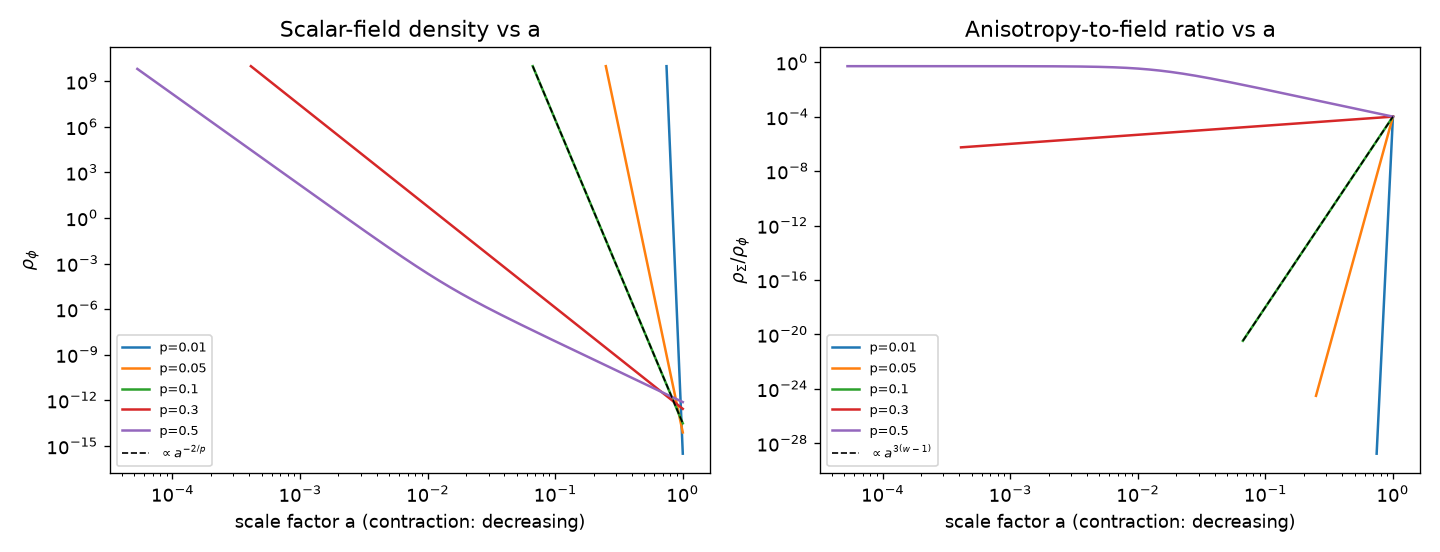
\includegraphics[width=\textwidth]{../results/figs/fig1_smoothing.png}
  \caption{\textbf{Contraction for different equations of state.}
  Left: scalar-field density vs scale factor for
  $p\in\{0.01,0.05,0.1,0.3,0.5\}$ (initial data on the attractor,
  $a(t_i)=1$; contraction proceeds to the left). Right: anisotropy ratio
  $\rhoSigma/\rhophi$ vs $a$. Dashed: analytic attractor slopes $a^{-2/p}$
  and $a^{3(w-1)}$. The $p=0.5$ curve ($w=1/3$) shows the ratio
  \emph{growing} as $a^{-2}$ until the shear leaves the perturbative
  regime.}
  \label{fig:smoothing}
\end{figure}

\begin{table}[b]
  \centering\small
  \caption{Fitted vs analytic exponents. Fits in the perturbative window
  $\rhoSigma/\rhophi<10^{-3}$; $R^2\ge0.99999999$; full data in
  \texttt{results/metrics.json}.}
  \label{tab:exponents}
  \begin{tabular}{ccccc}
    \toprule
    $p$ & $w$ & $\rhophi\propto a^{-3(1+w)}$: fit / theory
        & $\rhoSigma/\rhophi\propto a^{3(w-1)}$: fit / theory \\
    \midrule
    0.01 & 65.67 & $-199.9999$ / $-200$   & $193.9999$ / $194$ \\
    0.05 & 12.33 & $-40.0000$ / $-40$     & $34.0000$ / $34$   \\
    0.10 & 5.67  & $-20.0000$ / $-20$     & $14.0000$ / $14$   \\
    0.30 & 1.22  & $-6.6665$ / $-6.6667$  & $0.6665$ / $0.6667$\\
    0.50 & 0.33  & $-4.0007$ / $-4$       & $-1.9993$ / $-2$   \\
    \bottomrule
  \end{tabular}
\end{table}

Figure~\ref{fig:smoothing} and Table~\ref{tab:exponents} summarise step 1.
Fitted power-law exponents (log-log least squares in the window
$\rhoSigma/\rhophi<10^{-3}$) reproduce the attractor predictions
$\rhophi\propto a^{-2/p}$ and $\rhoSigma/\rhophi\propto a^{3(w-1)}$ to 4--6
significant digits.

Two points deserve emphasis. First, the $p=0.5$ run is a genuine
counterexample, not a failed simulation: $\rhoSigma/\rhophi\propto a^{-2}$
initially, the shear grows relative to the field, backreacts, and
eventually takes over the contraction entirely (Kasner-like domination).
The condition for smoothing is $w>1$, not contraction. Second, the
ekpyrotic phase is \emph{short}: the end of the physically relevant
contraction, at density $\rho_f$, occurs after
$n=\frac{p}{2}\ln(\rho_f/\rho_i)$ e-folds---here only $1.51$ e-folds to
reach $\rho=0.41$ for $p=0.1$. Smoothing nonetheless succeeds with ease:
from $f=10^{-4}$ the ratio falls by a factor $6.4\times10^{-10}$ over
those 1.5 e-folds, precisely because the suppression per e-fold
$e^{-3(w-1)}$ is enormous for $w\gg1$. This exponential-in-$\mathcal N$
structure, shared with the classicality result of
Sec.~\ref{sec:classicality}, is the operative fact, not the number of
e-folds.

\subsection{Anisotropy sensitivity and convergence}
\label{sec:convergence}

\begin{figure}[t]
  \centering
  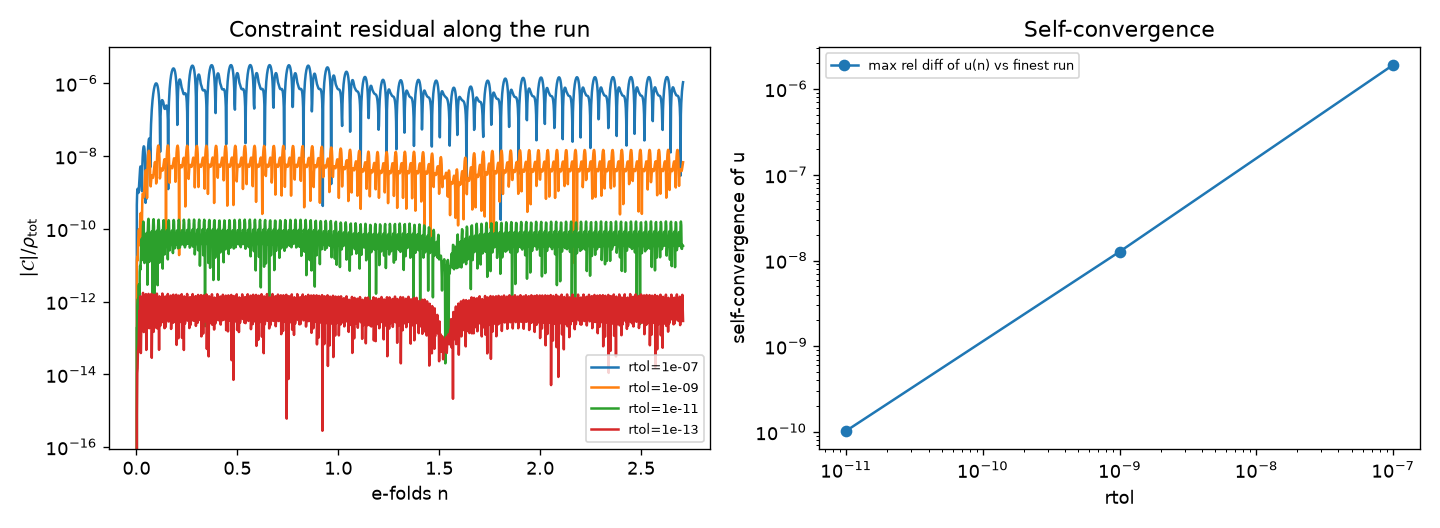
\includegraphics[width=\textwidth]{../results/figs/fig2_convergence.png}
  \caption{\textbf{Numerical control.} Left: independent Friedmann
  constraint residual $|\mathcal C|/\rho_{\rm tot}$ along the run ($p=0.1$,
  in e-fold time) at four tolerance levels. Right: self-convergence of
  $u(n)$ against the finest run, showing $\sim2$ digits gained per decade
  of relative tolerance.}
  \label{fig:convergence}
\end{figure}

Figure~\ref{fig:convergence} shows the tolerance sweep. The constraint
residual scales with the tolerance as expected
($3.2\times10^{-6}\to1.7\times10^{-12}$ relative to $\rho_{\rm tot}$ for
rtol $10^{-7}\to10^{-13}$), and the fitted smoothing exponent is stable at
$13.99998$ (theory $14$) at all but the loosest tolerance.

Parameter sensitivity: varying the initial shear fraction over
$f\in\{10^{-6},10^{-4},10^{-2}\}$ leaves the exponent unchanged
($14.000000$, $13.999978$, $13.997786$) and the final ratio scales
linearly, $\{3.420,3.420,3.434\}\times10^{-23,-21,-19}$: a $1\%$ shear
fraction at three decades below Planckian cutoff still leaves a sub-percent
ratio at the cutoff. Varying $V_0$ over two decades changes nothing
($13.999978$ throughout), as expected since $V_0$ only redefines
$\phi_i$.

\subsection{GR contraction versus a specified effective bounce}
\label{sec:bounce}

\begin{figure}[t]
  \centering
  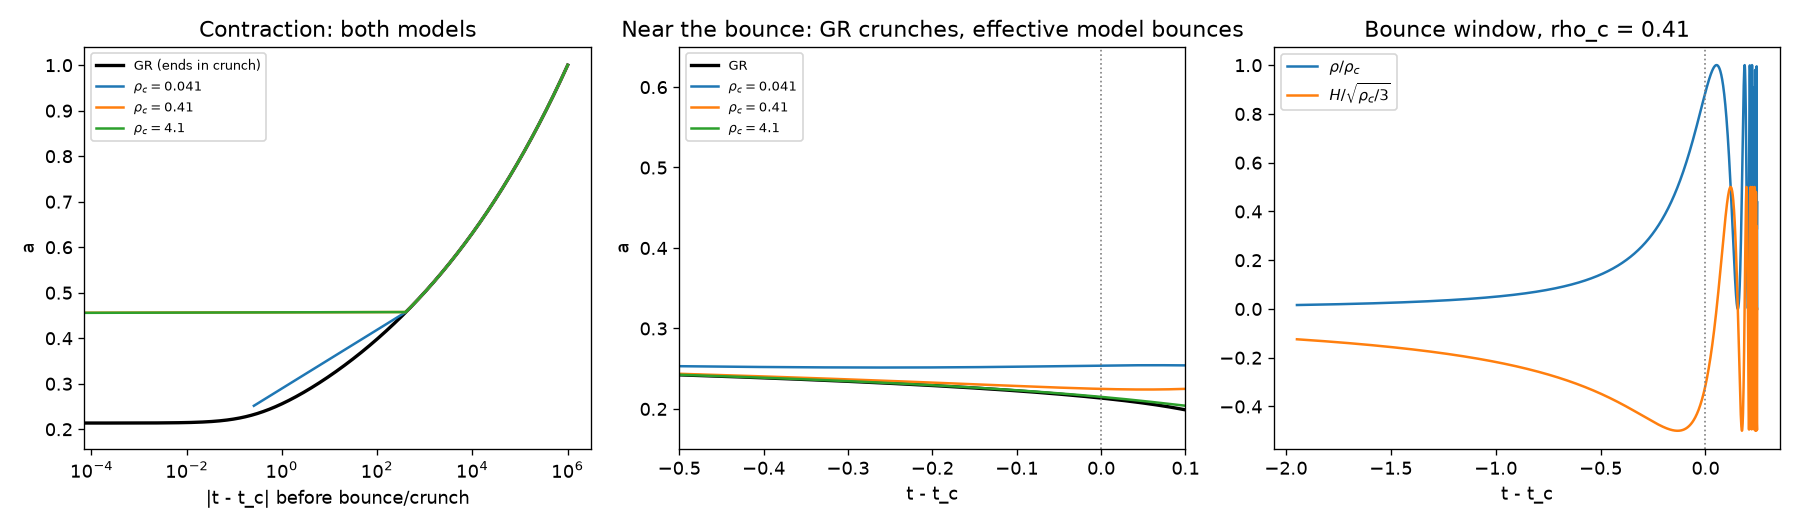
\includegraphics[width=\textwidth]{../results/figs/fig3_bounce.png}
  \caption{\textbf{No bounce versus specified bounce.} Left: $a$ against
  time $|t-t_c|$ to crunch (GR) and to bounce (effective model,
  $\rhoc/0.41\in\{0.1,1,10\}$); the curves are indistinguishable until
  $\rho\sim\rhoc$. Middle: the same solutions near the high-density region
  (crunch-centred time, see Sec.~\ref{sec:marginal}); the effective model
  bounces, the GR solution ends. Right: $\rho/\rhoc$ and
  $H/\sqrt{\rhoc/3}$ for $\rhoc=0.41$ through the bounce: the expanding
  branch recollapses ($\rho\to0$) and, if continued, the model enters a
  cascade of bounces accumulating in finite time---the region of densely
  packed features at the right edge, which we treat as a breakdown of the
  ad-hoc dynamics.}
  \label{fig:bounce}
\end{figure}

\begin{table}[b]
  \centering\small
  \caption{Bounce locations ($p=0.1$). $\rho(t_b)=\rhoc$ holds to ten
  digits in every case. $a_{\rm GR}(\rhoc)$ is the GR scale factor at the
  same density; the suppression column uses the GR scaling
  \eqref{eq:smoothing} up to that density.}
  \label{tab:bounce}
  \begin{tabular}{cccc}
    \toprule
    $\rhoc$ & $a_{\rm bounce}$ & $a_{\rm GR}(\rhoc)$
    & $\rhoSigma/\rhophi$ suppression up to $\rho=\rhoc$\\
    \midrule
    0.041 & 0.2513 & 0.2473 & $2.0\times10^{-9}$  \\
    0.41  & 0.2240 & 0.2204 & $6.4\times10^{-10}$ \\
    4.1   & 0.1996 & 0.1964 & $2.0\times10^{-10}$ \\
    \bottomrule
  \end{tabular}
\end{table}

The GR solution crunches. The specified dynamics
\eqref{eq:eff-friedmann}, \eqref{eq:eff-ray}, starting from identical
initial data, follows it exactly until $\rho$ approaches $\rhoc$ and then
bounces---cleanly, at $\rho=\rhoc$ to ten digits
(Table~\ref{tab:bounce}). The bounce occurs at essentially the scale factor
at which GR reaches the same density ($a_b/a_{\rm GR}$ within $2\%$; the
difference is the modified source term acting over the densest stretch of
the contraction).

The more informative result is what happens \emph{after} the bounce. The
potential being negative, the expanding branch cannot persist: the kinetic
energy redshifts as $a^{-6}$ and catches up with $|V|$ almost at once; the
model recollapses after expanding by only
\begin{equation}
  \frac{a_{\max}}{a_{\rm bounce}}\;=\;1.0115 \qquad (\rhoc=0.41,\ p=0.1).
  \label{eq:expansion}
\end{equation}
Continued further, the effective dynamics falls into a cascade of
contraction--bounce--recollapse cycles whose period shrinks fast enough
for an infinite number of bounces to accumulate at a finite time
(Fig.~\ref{fig:bounce}, right). We classify the cascade as an artifact: it
signposts the point where gluing \eqref{eq:eff-friedmann} onto a negative
exponential potential with unchanged continuity stops being a model. In
realistic ekpyrotic constructions the bounce mechanism explicitly
\emph{changes} the dynamics in the high-energy phase (ghost condensation
violates the null energy condition~\cite{Buchbinder:2007ad}; galileon
bounces modify the kinetic sector~\cite{Easson:2011zy}); none of that
machinery is present here, and the cascade is the price.

The positive content of this comparison: (i) the bounce in the specified
model lands exactly where it should, which validates the implementation;
(ii) smoothing is long finished before the bounce ($\sim10^{9}$ suppression
by $\rho=\rhoc$), so the post-bounce isotropy is inherited, not generated,
by the bounce model; (iii) the failure mode is sharp and visible---which is
the reason for including a model we know to be incomplete.

\subsection{WKB classicality along the ekpyrotic branch}
\label{sec:classicality}

\begin{figure}[t]
  \centering
  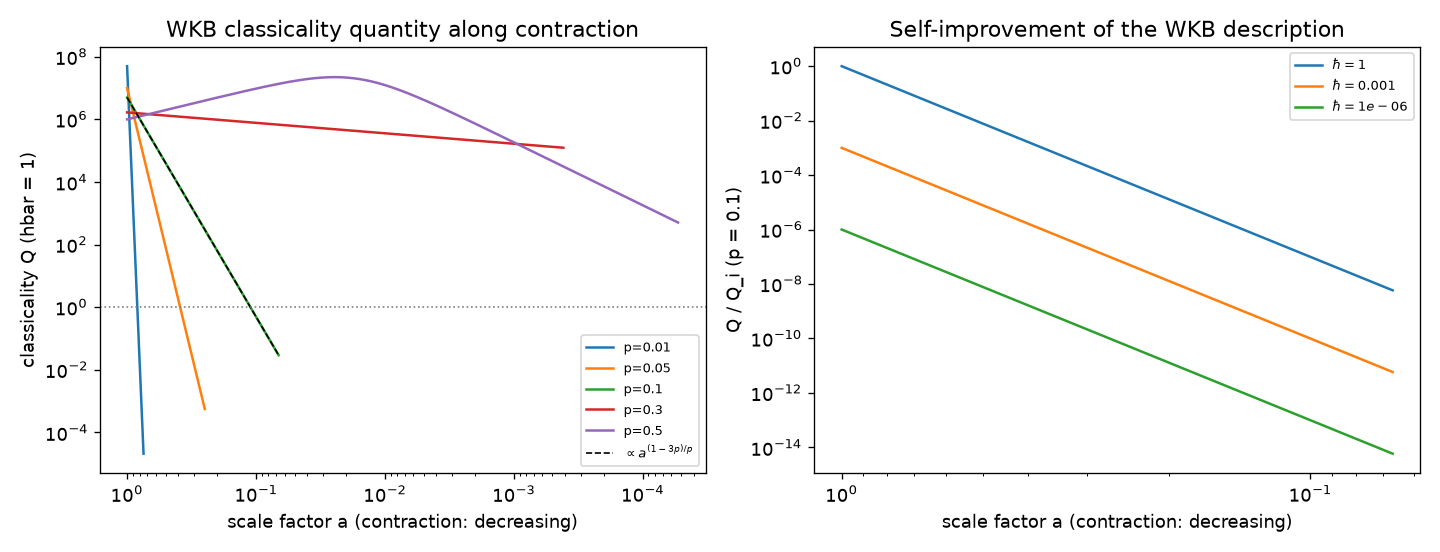
\includegraphics[width=\textwidth]{../results/figs/fig4_classicality.png}
  \caption{\textbf{Classicality.} Left: $\cQ(a)$ along the contraction for
  the five equations of state ($\hbar=1$); dashed, the attractor slope
  $a^{(1-3p)/p}$. For $p<1/3$ the WKB description improves monotonically as
  the high-density region is approached; for $p=0.5$ ($w<1$) it degrades as
  the shear takes over. Right: same run ($p=0.1$), normalised, for three
  values of the overall $\hbar$ factor: the exponent is $\hbar$
  independent, the overall level is not.}
  \label{fig:classicality}
\end{figure}

\begin{table}[b]
  \centering\small
  \caption{WKB classicality: fitted exponent of $\cQ(a)$ vs the attractor
  prediction $(1-3p)/p$; $\cQ$ at the initial slice and at the GR trust
  cutoff ($\hbar=1$).}
  \label{tab:Q}
  \begin{tabular}{cccc}
    \toprule
    $p$ & fit / theory & $\cQ(t_i)$ & $\cQ(\rho_{\rm stop})$\\
    \midrule
    0.01 & $96.99997$ / $97$  & $5.0\times10^{7}$ & $2.1\times10^{-5}$\\
    0.05 & $16.99999$ / $17$  & $1.0\times10^{7}$ & $5.6\times10^{-4}$\\
    0.10 & $6.99999$ / $7$    & $5.0\times10^{6}$ & $2.9\times10^{-2}$\\
    0.30 & $0.33334$ / $0.33333$ & $1.7\times10^{6}$ & $1.2\times10^{5}$\\
    0.50 & $-0.9972$ / $-1$   & $1.0\times10^{6}$ & $5.1\times10^{2}$\\
    \bottomrule
  \end{tabular}
\end{table}

Figure~\ref{fig:classicality} shows $\cQ$ computed from the numerical
trajectory via \eqref{eq:Q}. The fitted power laws match the attractor
prediction \eqref{eq:Qscaling} to 4--6 digits for all $p$
(Table~\ref{tab:Q}). For ekpyrotic $p$, $\cQ$ plummets: with $\hbar=1$ in
our units, $\cQ(t_i)\sim5\times10^6$ falls below $1$ at
$a/a_i\approx0.11$ for $p=0.1$. The $w<1$ run degrades classicality
($\cQ\propto a^{-1}$ in the perturbative window), consistent with the
picture that what fails to smooth also fails to
classicalise~\cite{Lehners:2015}.

As derived in Sec.~\ref{sec:model}, our measured exponent is exactly the
classicality factor $e^{-(\epsilon-3)\mathcal N/(\epsilon-1)}$ of
Ref.~\cite{Lehners:2015}. Two caveats delimit what this establishes.
First, $\cQ\propto\hbar$ (it is the ratio of the transport to the
Hamilton--Jacobi equation): the \emph{exponent} is convention independent,
the crossing point of $\cQ=1$ is not, and we quote $\hbar=1$ explicitly.
Second, \eqref{eq:Q} is a self-consistency criterion for a WKB state peaked
on the given classical history in minisuperspace (first-derivative-free
factor ordering, no fluctuations); it does not select among boundary
proposals, nor address the quantum production of perturbations---the parts
of the classicality debate carried, in Refs.~\cite{Lehners:2015,
BattarraLehners:2014,Feldbrugge:2017}, by saddle-point analyses of the
wavefunction. What we verify here is the local dynamical input to those
analyses: along the ekpyrotic history the WKB ansatz improves precisely as
predicted, throughout the phase.

%====================================================================
\section{Attractor stability, and why naive bounce continuations fail}
\label{sec:stability}
%====================================================================

\subsection{Exact spectrum in $t$-invariant relative coordinates}
\label{sec:spectrum}

The convergence of the contraction onto the scaling solution, and the
marginal behaviour of Sec.~\ref{sec:marginal}, are both captured exactly by
a change of variables. For the pure-scalar system ($\rhoSigma=0$) define
\begin{equation}
  X=-c\,(\phi-\phi_{\rm att}),\qquad
  U=\frac{u}{u_{\rm att}(n)},\qquad
  H_h=\frac{h}{h_{\rm att}(n)},
  \label{eq:scaled}
\end{equation}
where $\phi_{\rm att}(n)=\phi_i-2n/(cp)$ and
$u_{\rm att},h_{\rm att}\propto e^{n/p}$ are the attractor slices. All
three are $t$-invariant relative coordinates, and the flow
\eqref{eq:system-n} reduces \emph{exactly} (not to linear order) to the
autonomous system
\begin{equation}
  \dot X=\frac{2}{p}\Bigl(\frac{U}{H_h}-1\Bigr),\qquad
  \dot U=\Bigl(3-\frac1p\Bigr)U+\frac{1-3p}{p}\,\frac{e^{X}}{H_h},\qquad
  \dot H_h=\frac{1}{p}\Bigl(\frac{U^2}{H_h}-H_h\Bigr),
  \label{eq:scaled-system}
\end{equation}
with fixed point $(X,U,H_h)=(0,1,1)$. Linearising there gives the exact
spectrum
\begin{equation}
  \lambda_0=0,\qquad
  \lambda_1=-\frac{1-3p}{p}=-\frac{3}{2}(w-1),\qquad
  \lambda_2=-\frac{2}{p}=-3(w+1),
  \label{eq:spectrum}
\end{equation}
all real; the numerical Jacobian reproduces \eqref{eq:spectrum} to eight
digits for every $p$ tested (Fig.~\ref{fig:stability}). Three readings:

\begin{itemize}
  \item $\lambda_0=0$ with eigenvector $(2,1,1)$: the time-translation
        direction, i.e.\ the marginal mode of Sec.~\ref{sec:marginal}. In
        these coordinates a time shift is exactly a constant offset---the
        only memory a converged solution retains.
  \item $\lambda_1=-\frac32(w-1)$: deviations decay as
        $a^{3(w-1)/2}$---\emph{exactly half the smoothing exponent}
        \eqref{eq:smoothing}. Measured on the full five-variable system for
        $p=0.1$ with a $1\%$ velocity perturbation: decay rate
        $6.99$--$7.00$ per e-fold against the theoretical $7.00$, identical
        in all three coordinates. For $w\gg1$ a fraction of one e-fold
        erases generic homogeneous perturbations.
  \item $\lambda_1=0\iff w=1$: the scaling solution is linearly
        \emph{unstable} precisely when $w<1$, where deviations grow as
        $a^{3(w-1)/2}\to\infty$ during contraction. The $w=1$ threshold
        thus plays a double role: it is both the smoothing condition
        \eqref{eq:smoothing} and the exact stability boundary of the
        dynamics that performs the smoothing. The $\lambda_2=-3(w+1)$ mode
        decays faster still and is numerically invisible after
        $\sim\!0.05$ e-folds.
\end{itemize}

\begin{figure}[t]
  \centering
  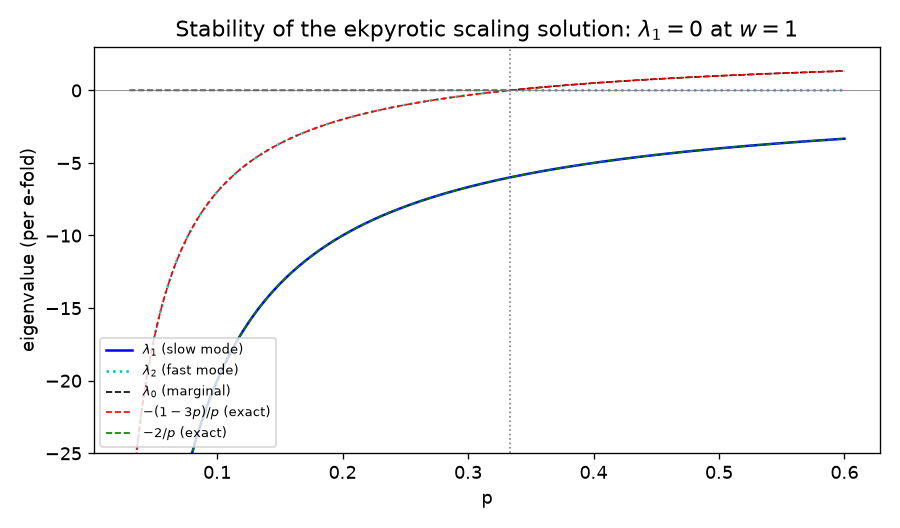
\includegraphics[width=0.72\textwidth]{../results/figs/fig5_stability.png}
  \caption{\textbf{Stability of the ekpyrotic scaling solution.} The two
  nonzero eigenvalues of \eqref{eq:spectrum} against $p$: numerical
  Jacobian (solid) and exact formulas (dashed) coincide. The slow mode
  $\lambda_1$ crosses zero exactly at $p=1/3$ ($w=1$): for $p>1/3$ the
  solution that would be doing the smoothing is itself unstable.}
  \label{fig:stability}
\end{figure}

\begin{figure}[t]
  \centering
  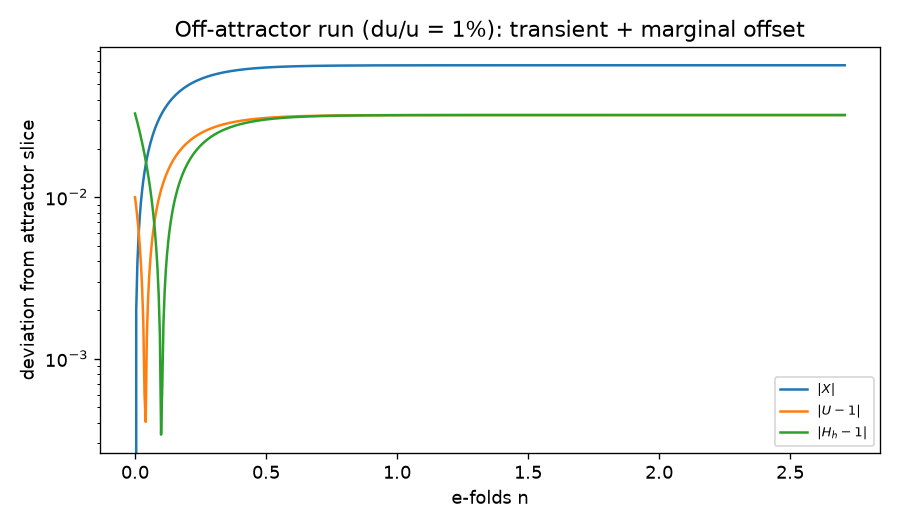
\includegraphics[width=0.72\textwidth]{../results/figs/fig6_convergence.png}
  \caption{\textbf{Convergence onto a shifted attractor.} Deviations of the
  three scaled coordinates from the attractor slice, for the full system
  with a $1\%$ velocity perturbation ($p=0.1$). Each curve is a decaying
  transient ($e^{-7n}$) on top of a constant offset---the marginal
  component, which is a pure time shift.}
  \label{fig:convergence2}
\end{figure}

\subsection{The Zeno cascade}
\label{sec:cascade}

\begin{figure}[t]
  \centering
  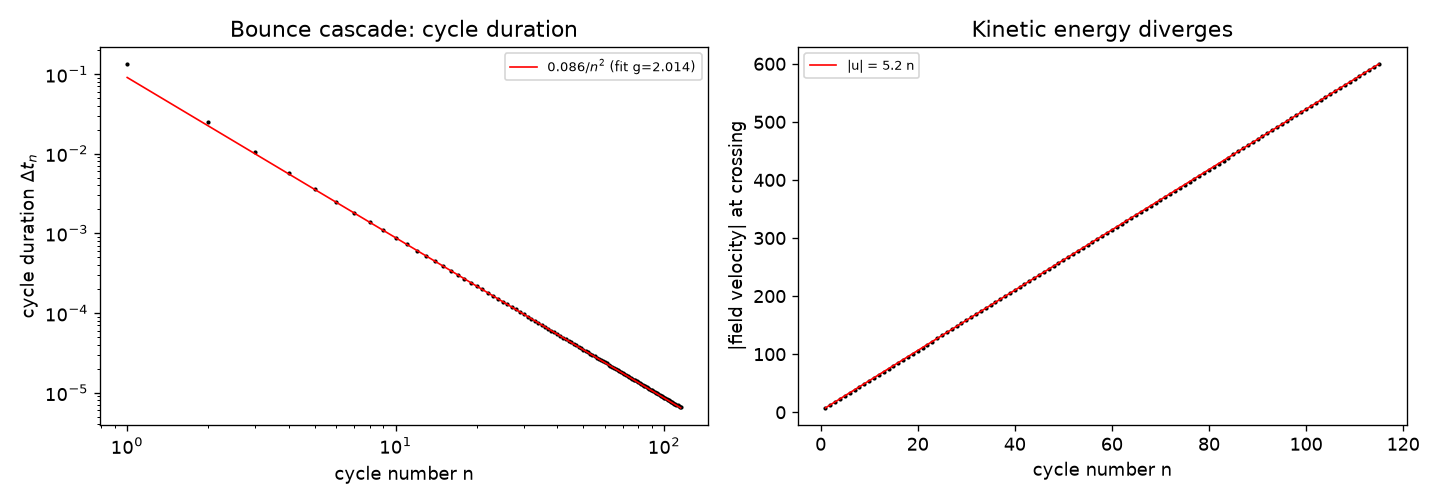
\includegraphics[width=\textwidth]{../results/figs/fig7_cascade.png}
  \caption{\textbf{The bounce cascade.} Left: cycle durations
  $\Delta t_n$ against cycle number, with the fitted law
  $\Delta t_n=0.086/n^{2.01}$. Right: field velocity at the crossings,
  $|u|_n=5.2\,n+2$. The $\sum n^{-2}$ series accumulates at
  $t_{\rm acc}\approx-3.6254$: infinitely many bounces with unbounded
  kinetic energy in finite time.}
  \label{fig:cascade}
\end{figure}

The recollapse that ends the expanding branch in
Sec.~\ref{sec:bounce} is itself degenerate: $\rho\to0$ requires
$\frac12u^2=|V|$ to high precision, and at the first recollapse the field
velocity has already grown to $u\approx-711$ against $|V|\approx2.5\times
10^5$ (our parameter values)---a mutual cancellation maintained to ten
digits by the constraint. Continuing the integration past it (with a floor
event at $\rho=10^{-8}\rhoc$), the effective dynamics generates a sequence
of bounce cycles whose durations follow
\begin{equation}
  \Delta t_n=\frac{A}{n^{2}},\qquad
  A=\frac{3p}{\pi\sqrt{3\rhoc}},
  \qquad |u|_n=\alpha n+\mathcal O(1),\quad
  \alpha=c\pi\sqrt{\tfrac{\rhoc}{3}} ,
  \label{eq:cascade}
\end{equation}
with the field gliding down the potential as $\phi_n=\phi_0-\tfrac{2}{c}
\ln n$. This law is not merely a fit: it is derivable in three steps,
asymptotically in $n$ (where $|V|\gg\rhoc$ at the turnarounds and $R$ is
negligible).

\emph{(i) Cycle time.} Along the effective flow $\rho+p=u^2$ and
$H=\sqrt{\rho(1-\rho/\rhoc)/3}$, so the time for one traversal
$\rhoc\to0$ (or $0\to\rhoc$) at approximately constant $u$ is
\begin{equation}
  T_{1/2}=\int_0^{\rhoc}\frac{\dd\rho}{3Hu^2}
  =\frac{1}{\sqrt3\,u^2}\int_0^{\rhoc}
     \frac{\dd\rho}{\sqrt{\rho(1-\rho/\rhoc)}}
  =\frac{\pi\sqrt{\rhoc/3}}{u^2},
  \label{eq:halfcycle}
\end{equation}
the $\rho$-integral being elementary ($\rho=\rhoc\sin^2\theta$); a full
bounce-to-bounce cycle doubles this.

\emph{(ii) Velocity growth.} Over a cycle, $\Delta u=\oint\dot u\,\dd t$
with $\dot u=-3Hu-c|V|$. The friction term integrates to
$-3\oint H\,\dd t=-3\,\Delta\ln a\simeq0$ ($a$ returns to its bounce
value), while $|V|$ is nearly constant across a cycle (the field moves by
only $\Delta\phi\sim1/u$). Using the turnaround constraint
$|V|=u^2/2-\rhoc+R\simeq u^2/2$, the $u^2$ \emph{cancels}:
\begin{equation}
  \Delta u\simeq-c\,|V|\,T=-c\,\frac{u^2}{2}\,
  \frac{2\pi\sqrt{\rhoc/3}}{u^2}
  =-c\pi\sqrt{\tfrac{\rhoc}{3}}\;\equiv\;-\alpha .
  \label{eq:alphagrowth}
\end{equation}

\emph{(iii) The law.} Substituting $u_n=\alpha n$ into the doubled
\eqref{eq:halfcycle} gives \eqref{eq:cascade} with
$A=2\pi\sqrt{\rhoc/3}/\alpha^2=3p/\pi\sqrt{3\rhoc}$: the exponent
$\gamma=2$ is \emph{exact}, and $A$ carries no free parameters. The field
drift follows as $\Delta\phi_n=\oint u\,\dd t\simeq-u_nT_n=-2/(cn)$, i.e.\
a harmonic (not geometric) creep, and the accumulation tail is
$t_{\rm acc}-t_N=A\,(\pi^2/6-H_N^{(2)})\simeq A/N$.

All four predictions are confirmed numerically (Fig.~\ref{fig:cascade} and
Fig.~\ref{fig:cascadelaw}): the growth rate $\alpha$ to four significant
digits for both $p=0.1$ ($5.1938$ vs $c\pi\sqrt{\rhoc/3}=5.1939$) and
$p=0.05$ ($7.3452$ vs $7.3453$); the scaled cycle time
$\Delta t_nu_n^2/2\pi\sqrt{\rhoc/3}=1.025\pm0.022$ and $1.026\pm0.022$
(the excess being the $1/n$ transient at small $n$); the drift law
$\Delta\phi_n/-2/(cn)=1.004$ and $1.002$; and the accumulation time from
the analytic tail sum, $t_{\rm acc}=-3.625382$, matching the earlier
series estimate. The $A\propto p$ scaling is also confirmed ($0.0443$
measured vs $0.0431$ predicted at $p=0.05$).

\begin{figure}[t]
  \centering
  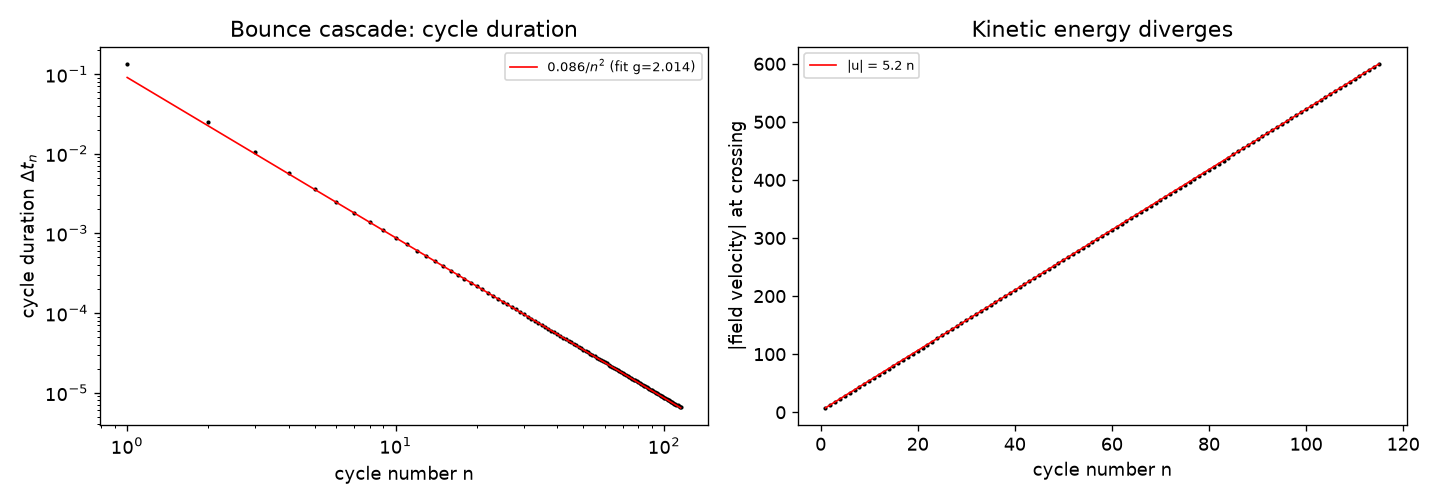
\includegraphics[width=\textwidth]{../results/figs/fig7_cascade.png}
  \caption{\textbf{The bounce cascade.} Left: cycle durations
  $\Delta t_n$ against cycle number, with the fitted law
  $\Delta t_n=0.086/n^{2.01}$. Right: field velocity at the crossings,
  $|u|_n=5.2\,n+2$. The $\sum n^{-2}$ series accumulates at
  $t_{\rm acc}\approx-3.6254$: infinitely many bounces with unbounded
  kinetic energy in finite time.}
  \label{fig:cascade}
\end{figure}

\begin{figure}[t]
  \centering
  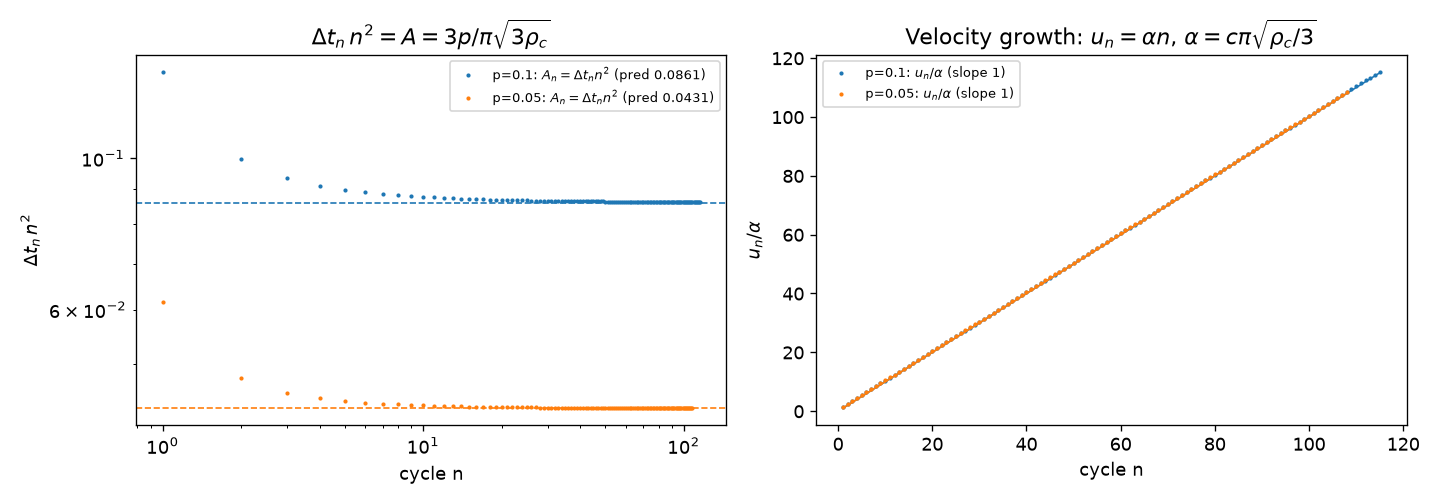
\includegraphics[width=\textwidth]{../results/figs/fig8_cascade_law.png}
  \caption{\textbf{The cascade law, derived vs measured.} Left:
  $\Delta t_n n^2$ converges onto the predicted $A=3p/\pi\sqrt{3\rhoc}$
  (dashed) for both $p$. Right: $u_n/\alpha$ is a unit-slope line,
  $\alpha=c\pi\sqrt{\rhoc/3}$, for both $p$.}
  \label{fig:cascadelaw}
\end{figure}

We emphasise that densities never leave $[0,\rhoc]$ in this sequence; it
is the velocity that diverges, which is why the breakdown is easy to miss
if one monitors only $\rho$. The cascade is thus a Zeno-type pathology of
the closure \eqref{eq:eff-friedmann} glued to a negative potential, now
with a quantitatively explained structure.

\subsection{A failed remedy: flipping the sign of the potential}
\label{sec:vflip}

A natural guess is that the recollapse is simply the fault of $V<0$, and
that letting the potential turn positive at the bounce (a crude stand-in
for reheating) would sustain the expansion. It does not. At the bounce the
field velocity is inherited from the contraction, $u_b=-2.44$, pointing
toward larger $|V|$; with $V>0$ in the expanding branch the field equation
keeps driving $\phi$ toward more negative values, $|V|=V_0e^{-c\phi}$
grows, and the on-shell solution is driven back across the constraint
boundary $\rho=\rhoc$ within $\Delta t\lesssim0.2$ of the bounce, where the
integration breaks down. Between the Zeno cascade ($V<0$) and this
runaway ($V>0$), the conclusion is that \emph{no} continuation of
\eqref{eq:eff-friedmann} with an unchanged scalar sector produces a valid
expanding phase: a working bounce must alter the field's post-bounce
roll---as the ghost-condensate mechanism of Ref.~\cite{Buchbinder:2007ad}
(asymptotic approach to the top of the potential) and galileon
constructions~\cite{Easson:2011zy} (modified kinetic sector) in fact do.

%====================================================================
\section{A marginal mode of the ekpyrotic attractor}
\label{sec:marginal}
%====================================================================

Our accuracy study exposed a conditioning property of the scaling solution
that matters for any numerical treatment of ekpyrotic backgrounds,
independent of the physics conclusions above. Its linear origin is the zero
eigenvalue of the spectrum \eqref{eq:spectrum}: the time-translation
direction, which is exactly marginal in the $t$-invariant variables.

The family \eqref{eq:attractor} has an exact time-translation symmetry:
given any solution, $t\to t+\delta t_c$ is another. Linearising about the
attractor, a homogeneous perturbation decomposes into stable directions
(decaying relative to the background as powers of $a$) plus the symmetry
direction, whose effect is to shift the time coordinate. In e-fold time the
background time behaves as $t_c-|t|=|t_c-t_i|e^{-n/p}$, so an initial
time offset appears as
\begin{equation}
  \delta t(n)=\delta t_{c,0}\,e^{n/p},
  \label{eq:marginal}
\end{equation}
i.e.\ the time-translation component is \emph{exactly marginal} in the
physical ($t$-invariant) variables---it neither grows nor decays relative
to the background---but appears as an exponentially growing offset in the
$t$ coordinate itself. Consequently, \emph{any} homogeneous perturbation of
the attractor---an offset of the initial data, or the small change in
$\dot H$ from the shear term---acquires a growing error in the measured
crunch time, while convergence to the attractor in all physical variables
is unaffected.

We verified this quantitatively by integrating the GR system in cosmic time
from attractor initial data with $H_i$ on the constraint surface and shear
fraction $f\in\{0,10^{-6},10^{-5},10^{-4},10^{-3}\}$: the displacement of
the measured crunch time is exactly linear,
\begin{equation}
  \frac{\delta t_c}{|t_i|}\simeq -36.8\,f \qquad (p=0.1),
  \label{eq:drift}
\end{equation}
over three decades of $f$, and independent of the integrator tolerance down
to rtol $10^{-13}$---it is the physical response of the homogeneous system
to shear backreaction, not solver noise. For $p=0.1$ and $f=10^{-4}$ the
crunch sits at $t_c\simeq-3.95$ instead of the unperturbed $-0.27$.

Two practical corollaries follow. First, comparisons between contracting
solutions (e.g.\ GR versus modified dynamics, as in
Sec.~\ref{sec:bounce}) must be made in crunch-centred time $t-t_c$ or,
better, in $t$-invariant variables ($a$, $n$, $\rho$); in absolute $t$, the
marginal mode masquerades as a genuine dynamical discrepancy. Second,
cosmic-time integration is intrinsically fragile deep in the contraction:
relative errors at the working-precision level excite the mode, and no
tolerance recovers the target $t_c$; e-fold time removes the issue for all
quantities except $t$ itself, and $t$ never carries physical information in
this problem.

%====================================================================
\section{Assumptions, predictions, and what is left open}
\label{sec:assumptions}
%====================================================================

\paragraph{Assumed without derivation.}
(i) flat slicing and a single canonical scalar with an exactly exponential
potential; (ii) homogeneous, adiabatically evolved shear (exact for
Bianchi~I; inhomogeneous anisotropies, with their growing $a^{-2}$-gradient
modes~\cite{Erickson:2003zm}, are excluded); (iii) the effective Friedmann
equation \eqref{eq:eff-friedmann}, specified in the style of LQC effective
dynamics with continuity unchanged, and no claim of derivation; (iv) the
first-derivative-free WDW factor ordering and the minisuperspace
truncation; (v) initial data exactly on the scaling attractor. Item (v) is
mild---the attractor is known analytically and our runs spot-check its
stability---but a systematic off-attractor initial-data sweep is listed
below as open.

\paragraph{What the models predict, as verified here.}
(1) Smoothing exponent $3(w-1)$ exactly; suppression linear in the initial
shear fraction, insensitive to $V_0$, completed within $\mathcal
O(1)$ e-folds for $w\gg1$. Generic homogeneous perturbations decay as
$a^{3(w-1)/2}$, retaining only a time shift; the scaling solution is
linearly stable iff $w>1$. (2) No GR bounce; a specified $H^2$-deformed
dynamics bounces exactly at $\rho=\rhoc$ and inherits the smoothed state,
but recollapses immediately for $V<0$ ($a_{\max}/a_b=1.0115$); its
continuation is a Zeno cascade ($\Delta t_n\propto n^{-2}$, $|u|_n\propto
n$) accumulating in finite time, and flipping the sign of the potential
does not avert breakdown. (3) WKB classicality exponent $(1-3p)/p$
exactly---equivalently $e^{-(\epsilon-3)\mathcal N/(\epsilon-1)}$---so the
contracting branch becomes arbitrarily classical, in the WKB sense, as the
density grows, for all $w>1$, and progressively fails to for $w<1$.

\paragraph{What remains unverified or open.}
(i) A viable post-bounce history: matching to a hot expanding phase
requires physics absent here (ghost-condensate/galileon-type bounce
mechanics, reheating, or a potential that turns positive); our effective
model demonstrates the failure mode explicitly rather than resolving it,
and Sec.~\ref{sec:vflip} shows the failure is robust to a sign flip of the
potential. (ii) The cascade law $\Delta t_n\propto n^{-2}$ of
Sec.~\ref{sec:cascade} is now derived analytically and verified to four
significant digits, including its $p$-scaling; what remains open there is
only the $1/n$ correction terms (the few-percent transient at small $n$). (iii) Perturbations across the bounce and the quantum
boundary proposal (no-boundary vs tunnelling, cf.\
\cite{BattarraLehners:2014,Feldbrugge:2017}): our
Sec.~\ref{sec:classicality} is a trajectory-level WKB check, the input
to---not a substitute for---the saddle-point analyses.
(iv) Inhomogeneous anisotropy gradients. (v) Off-attractor initial data in
the anisotropic sector: Sec.~\ref{sec:spectrum} settles the pure-scalar
case (decay at $3(w-1)/2$ plus a time shift); the corresponding statement
with mixmaster-type shear excitations is open.

%====================================================================
\section{Conclusions}
%====================================================================

Within its stated assumptions, the classical ekpyrotic mechanism is exactly
what it claims to be: contraction with $w>1$ drives the universe to an
isotropic, scalar-dominated attractor, with the anisotropy ratio suppressed
as $a^{3(w-1)}$, to numerical precision far beyond what is physically
relevant, and within a handful of contraction e-folds. The dynamics is
even better behaved than the smoothing law alone suggests: in
$t$-invariant relative coordinates the flow about the attractor has the
exact spectrum $\{0,-\frac32(w-1),-3(w+1)\}$, so generic homogeneous
perturbations die as $a^{3(w-1)/2}$ within a fraction of an e-fold, and the
only memory they leave is a time shift---while for $w<1$ the same spectrum
turns unstable, the $w=1$ threshold thus governing both smoothing and
stability. Neither the contraction nor the smoothing contains an exit:
reading a bounce out of the background requires wholesale new dynamics, and
the naive option---an $H^2$-deformation glued onto the unchanged
negative-potential model---works exactly once and then visibly falls apart,
recollapsing into a Zeno cascade whose law we derive and confirm ($\Delta
t_n=3p\,n^{-2}/\pi\sqrt{3\rhoc}$, $|u|_n=c\pi\sqrt{\rhoc/3}\,n$: infinite
bounces with unbounded kinetic energy in finite time) that no sign flip of
the potential averts. Semiclassically, the
contracting branch is an increasingly good WKB history:
$\cQ\propto a^{(1-3p)/p}$ improves monotonically through ekpyrosis,
exponentially in the contraction e-folds, providing the local,
trajectory-level confirmation of the classicality behaviour found in the
no-boundary analyses of Ref.~\cite{Lehners:2015}. Finally, we have
quantified a numerical property of the ekpyrotic attractor with practical
consequences beyond this study: its marginal time-translation mode
amplifies any homogeneous perturbation into a strictly linear
crunch-time displacement, $\delta t_c\propto f$, which dictates the choice
of integration variables and warns against absolute-time comparisons of
contracting solutions.

%====================================================================
\begin{thebibliography}{99}
%====================================================================

\bibitem{Khoury:2001wf}
  J.~Khoury, B.~A.~Ovrut, P.~J.~Steinhardt and N.~Turok,
  \emph{The ekpyrotic universe: Colliding branes and the origin of the hot
  big bang}, Phys.\ Rev.\ D \textbf{64}, 123522 (2001)
  [arXiv:hep-th/0103239].

\bibitem{Erickson:2003zm}
  J.~K.~Erickson, D.~H.~Wesley, P.~J.~Steinhardt and N.~Turok,
  \emph{Kasner and mixmaster behavior in universes with equation of state
  $w\ge1$}, Phys.\ Rev.\ D \textbf{69}, 063514 (2004)
  [arXiv:hep-th/0312009].

\bibitem{Buchbinder:2007ad}
  E.~I.~Buchbinder, J.~Khoury and B.~A.~Ovrut,
  \emph{New ekpyrotic cosmology}, Phys.\ Rev.\ D \textbf{76}, 123503
  (2007) [arXiv:hep-th/0702154].

\bibitem{Easson:2011zy}
  D.~A.~Easson, I.~Sawicki and A.~Vikman,
  \emph{G-bounce}, JCAP \textbf{11}, 021 (2011) [arXiv:1109.1047].

\bibitem{Lehners:2008vx}
  J.-L.~Lehners,
  \emph{Ekpyrotic and cyclic cosmology}, Phys.\ Rept.\ \textbf{465}, 223
  (2008) [arXiv:0806.1245].

\bibitem{Lehners:2015}
  J.-L.~Lehners,
  \emph{Classical inflationary and ekpyrotic universes in the no-boundary
  wavefunction}, Phys.\ Rev.\ D \textbf{91}, 083525 (2015)
  [arXiv:1502.00629].

\bibitem{BattarraLehners:2014}
  L.~Battarra and J.-L.~Lehners,
  \emph{On the no-boundary proposal for ekpyrotic and cyclic cosmologies},
  JCAP \textbf{12}, 023 (2014) [arXiv:1407.4814].

\bibitem{Feldbrugge:2017}
  J.~Feldbrugge, J.-L.~Lehners and N.~Turok,
  \emph{No smooth beginning for spacetime}, Phys.\ Rev.\ Lett.\
  \textbf{119}, 171301 (2017) [arXiv:1705.00192].

\bibitem{Ashtekar:2006wn}
  A.~Ashtekar, T.~Pawlowski and P.~Singh,
  \emph{Quantum nature of the big bang}, Phys.\ Rev.\ Lett.\ \textbf{96},
  141301 (2006) [arXiv:gr-qc/0602086].

\bibitem{code}
  Origin Datum Math OS, task OD-QC-001 companion code repository:
  \texttt{src/ekpyrotic.py} (model and integrators),
  \texttt{notebooks/OD-QC-001\_ekpyrotic\_classicality.ipynb} (executed
  notebook producing every number and figure of this paper),
  \texttt{results/metrics.json} (machine-readable outputs).

\end{thebibliography}

\end{document}
